\chapter{Kubernetes}
\label{kubernetes}

\newcommand{\gluster}{GlusterFS}

In this appendix we provide a basic summary to the Kubernetes concepts and
we will show a simple way to perform a basic installation. This is not thought 
as an complete overview of functionalities but there are only reported a 
description of concepts an features used in the implementation of our solution. 

\section{Kubernetes basic concepts}
\label{kubernetes-basic-concepts}

\subsection{Pod}
\label{pod}

A Pod is the most basic building block for Kubernetes. Pods wrap up the
underlying virtualization technology used: in case its a container based
solution, it can contain one or more container (although this configuration is
worth only if the containers are highly coupled). Pods have a lifecycle, and
they can assume these states\footnote{
  \url{https://kubernetes.io/docs/concepts/workloads/pods/pod-lifecycle/}}:

\begin{description}
\item[Pending] The Pod has been accepted by the Kubernetes system, but
  one or more container images have not been created yet. This includes the Pod
  scheduling and image downloading which could take a while.
\item[Running] The Pod has been bound to a node, and all of the
  Containers have been created. At least one container is still running, or is
  in the process of starting or restarting.
\item[Succeeded] All containers in the Pod have terminated with
  success, and they will not be restarted.
\item[Failed] All containers in the Pod have terminated, and at least
  one container has terminated with a failure. That is, the container either
  exited with non-zero status or was terminated by the system.
\item[Unknown] For some reason the state of the Pod could not be
  obtained, typically due to an error communicating with the host of the Pod.
\end{description}

A Pod can have different conditions too:

\begin{description}
\item[PodScheduled] The Pod has been scheduled to a node;
\item[Ready]: the Pod is able to serve requests and should be added
  to the load balancing pools of all matching Services;
\item[Initialized] All init containers\footnote{
  \url{https://kubernetes.io/docs/concepts/workloads/pods/init-containers}}
  have started successfully;
\item[Unschedulable] The scheduler cannot schedule the Pod right
  now, for example due to the lacking of resources or other constraints;
\end{description}

Each Pod can have different QoS classes:
\begin{description}
  \item [Guaranteed] Every container in the Pod must have a memory and CPU
  limits and memory and CPU requests, and they must be the same;
  \item [Burstable] The Pod does not meet the criteria for QoS class
  Guaranteed and at least one container in the Pod has a memory or CPU request;
  \item [BestEffor] The containers in the Pod must not have any memory or CPU
  limits or requests.
\end{description}

\subsection{Service}
\label{service}

Since Pods for their nature are highly volatile, applications that use them can
not rely on their IP address. To solve this problem, the Service implementation
in Kubernetes assure a stable IP, even if different Pods in this service crash
and gets restarted by a ReplicaSet (which will not be explain in this appendix,
but it basically scale up and down Pods\footnote{
  \url{https://kubernetes.io/docs/concepts/workloads/controllers/replicaset/}}).
Citing the official documentation\footnote{
\url{https://kubernetes.io/docs/concepts/services-networking/service/}}, a
Service is:\\
\textquote{A Kubernetes Service is an abstraction which defines a logical set
of Pods and a policy by which to access them - sometimes called a
micro-service.}

\begin{figure}[htbp]
\centering
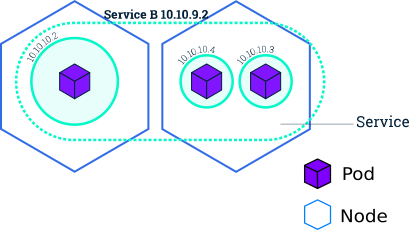
\includegraphics{k8s_services}
\caption{Example of a service}
\end{figure}

\subsection{Volume}
\label{volume}

When Pods saves data on a node, this information is designated to perish.
Kubernetes offers a way to save all the data and to possibly make it available
to all the Pods replicas, offering a transparent layer where Pods are not aware
of working with information shared other Pods, even located in other nodes. This
functionality is called Volume, and there are many different drivers, that range
from a simple local storage to \emph{\gluster{}}.

\subsection{Namespace}
\label{namespace}

Namespaces are intended to be used when there are multiple users accessing the
cluster, or to separate multiple projects.

\section{Kubernetes architectural concepts}
\label{kubernetes-architectural-concepts}

\subsection{Node}\label{node}

A node is the building block for a Kubernetes cluster. Everyone must have
at least the kubelet daemon (to manage Kubernetes functionalities) and a
container manager (e.g. Docker Engine, VirtualBox) running. A node runs Pods
and can communicate with other nodes in the same cluster.

\begin{figure}[htbp]
\centering
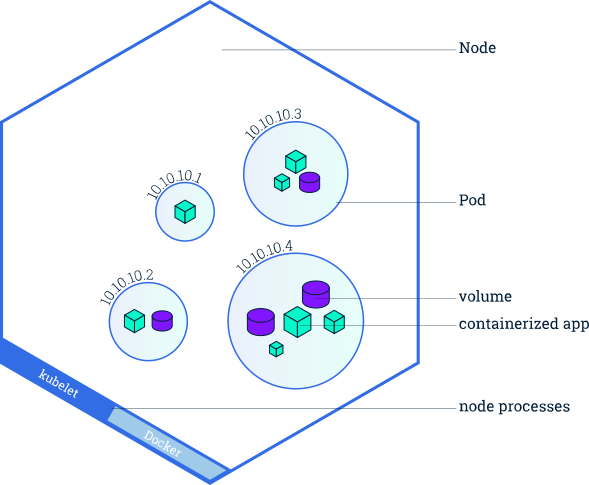
\includegraphics[scale=0.8]{k8s_nodes}
\caption{Schema illustrating the elements in a node}
\end{figure}

\subsection{Master}
\label{master}

The \emph{master node} is the one that starts a cluster, and that manage the
slaves. Only some Pods can run in the master node (e.g. the dashboard).

The master generates the token for the slaves to join, and eventually
coordinates the federation with other clusters. In a cluster, there is the
possibility to have multiple master to ensure high availability.

\subsection{Slave}
\label{slave}

A \emph{slave}, or \emph{minion} is a node that runs the Pods that the master
schedule. It can also be part of a \emph{PersistantVolume} storage (like
\gluster{}) and if it goes down, another slave will take care of the Pods that
where running on it. Minions can join an existing cluster via a given token.

\subsection{Networking}
\label{networking}

Kubernetes has its own networking structure, even if it uses Docker for running
containers. In particular, it delegates the network operations (like packet
forwarding) to different managers, such as Flannel or Calico.

Every node in the cluster runs a Pod called \texttt{kubeproxy}, that
communicates with the \texttt{kube-api} Pod (running on master) and
\texttt{kube-dns} (for Kubernetes \textless{}=1.9.x) or \texttt{CoreDNS} (for
Kubernetes \textgreater{}=1.10.x) services. \texttt{kubeproxy} assure
transparent communications between Pods in the same cluster, and
\texttt{kube-api} allows to call Kubernetes services. \texttt{kube-dns/CoreDNS}
manage DNS requests coming from the Pods, differentiating the one that goes
outside the cluster from the other that points internally\footnote{Additional
  information about Flannel, Kubernetes and Docker networking can at:\\\sloppy
  \url{https://www.sdxcentral.com/cloud/containers/definitions/what-is-coreos-flannel-definition/}}.

\begin{figure}[htbp]
\centering
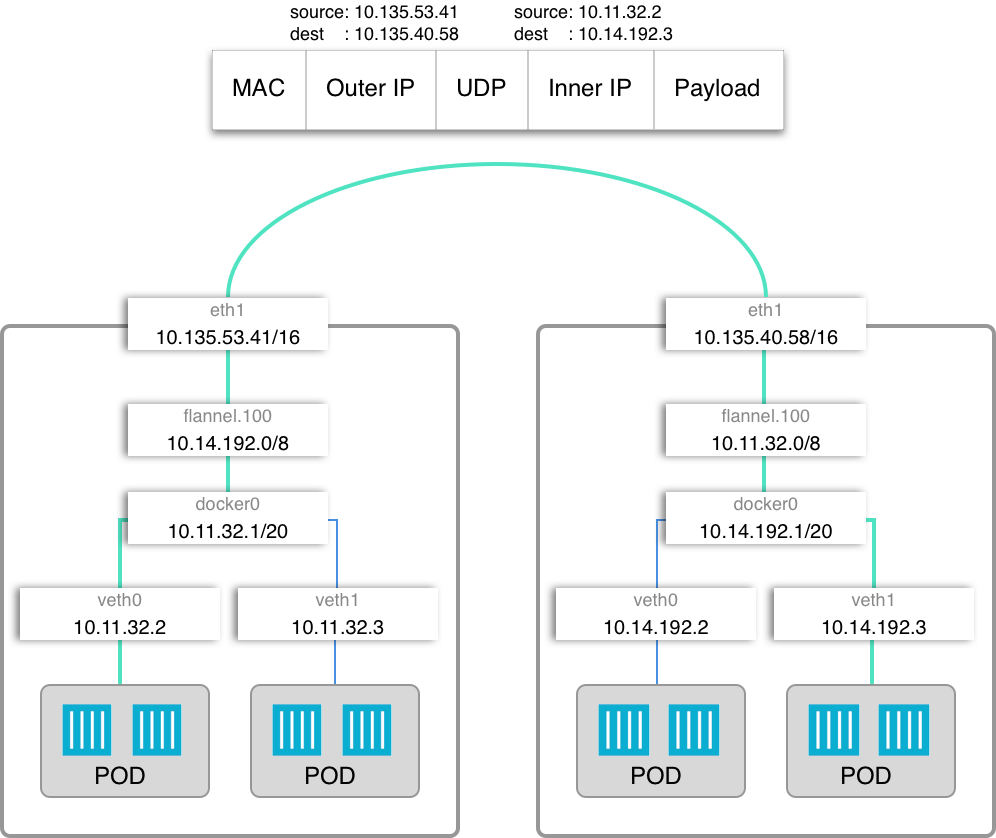
\includegraphics[scale=0.3]{flannelredirect}
\caption{And example of how Flannel redirects packages between Pods}
\end{figure}



\section{Focusing on Storage}
\label{focusing-on-storage}

This section is based on official Kubernetes documentation\footnote{%
  \url{https://kubernetes.io/docs/concepts/storage/persistent-volumes/}} and
from the \texttt{newstack site}\footnote{\sloppy
  \url{https://thenewstack.io/strategies-running-stateful-applications-kubernetes-persistent-volumes-claims/}}.

\subsection{Volumes, Claims and Classes}
\label{volumes-claims-and-classes}

Managing compute and storage resources are totally different problems and in
order to create a proper storage abstraction Kubernetes relies on the
\textbf{PersistantVolume} and the \textbf{PersistantVolumeClaim} features.

A PersistantVolume (PV) is something similar to a node, in fact is a piece of
storage provided by the administrator: it captures the details of the
implementation of the storage and has a lifecycle that is independent of any
individual Pod. To not expose developers to storage boring details admins can
expose different PV types through \textbf{StorageClasses}.

A PersistantVolumeClaim (PVC) instead is a request for storage and it is similar
to a Pod: instead of requesting memory and CPU, a PVC requests certain size and
access mode to storage.

\begin{figure}[htbp]
\centering
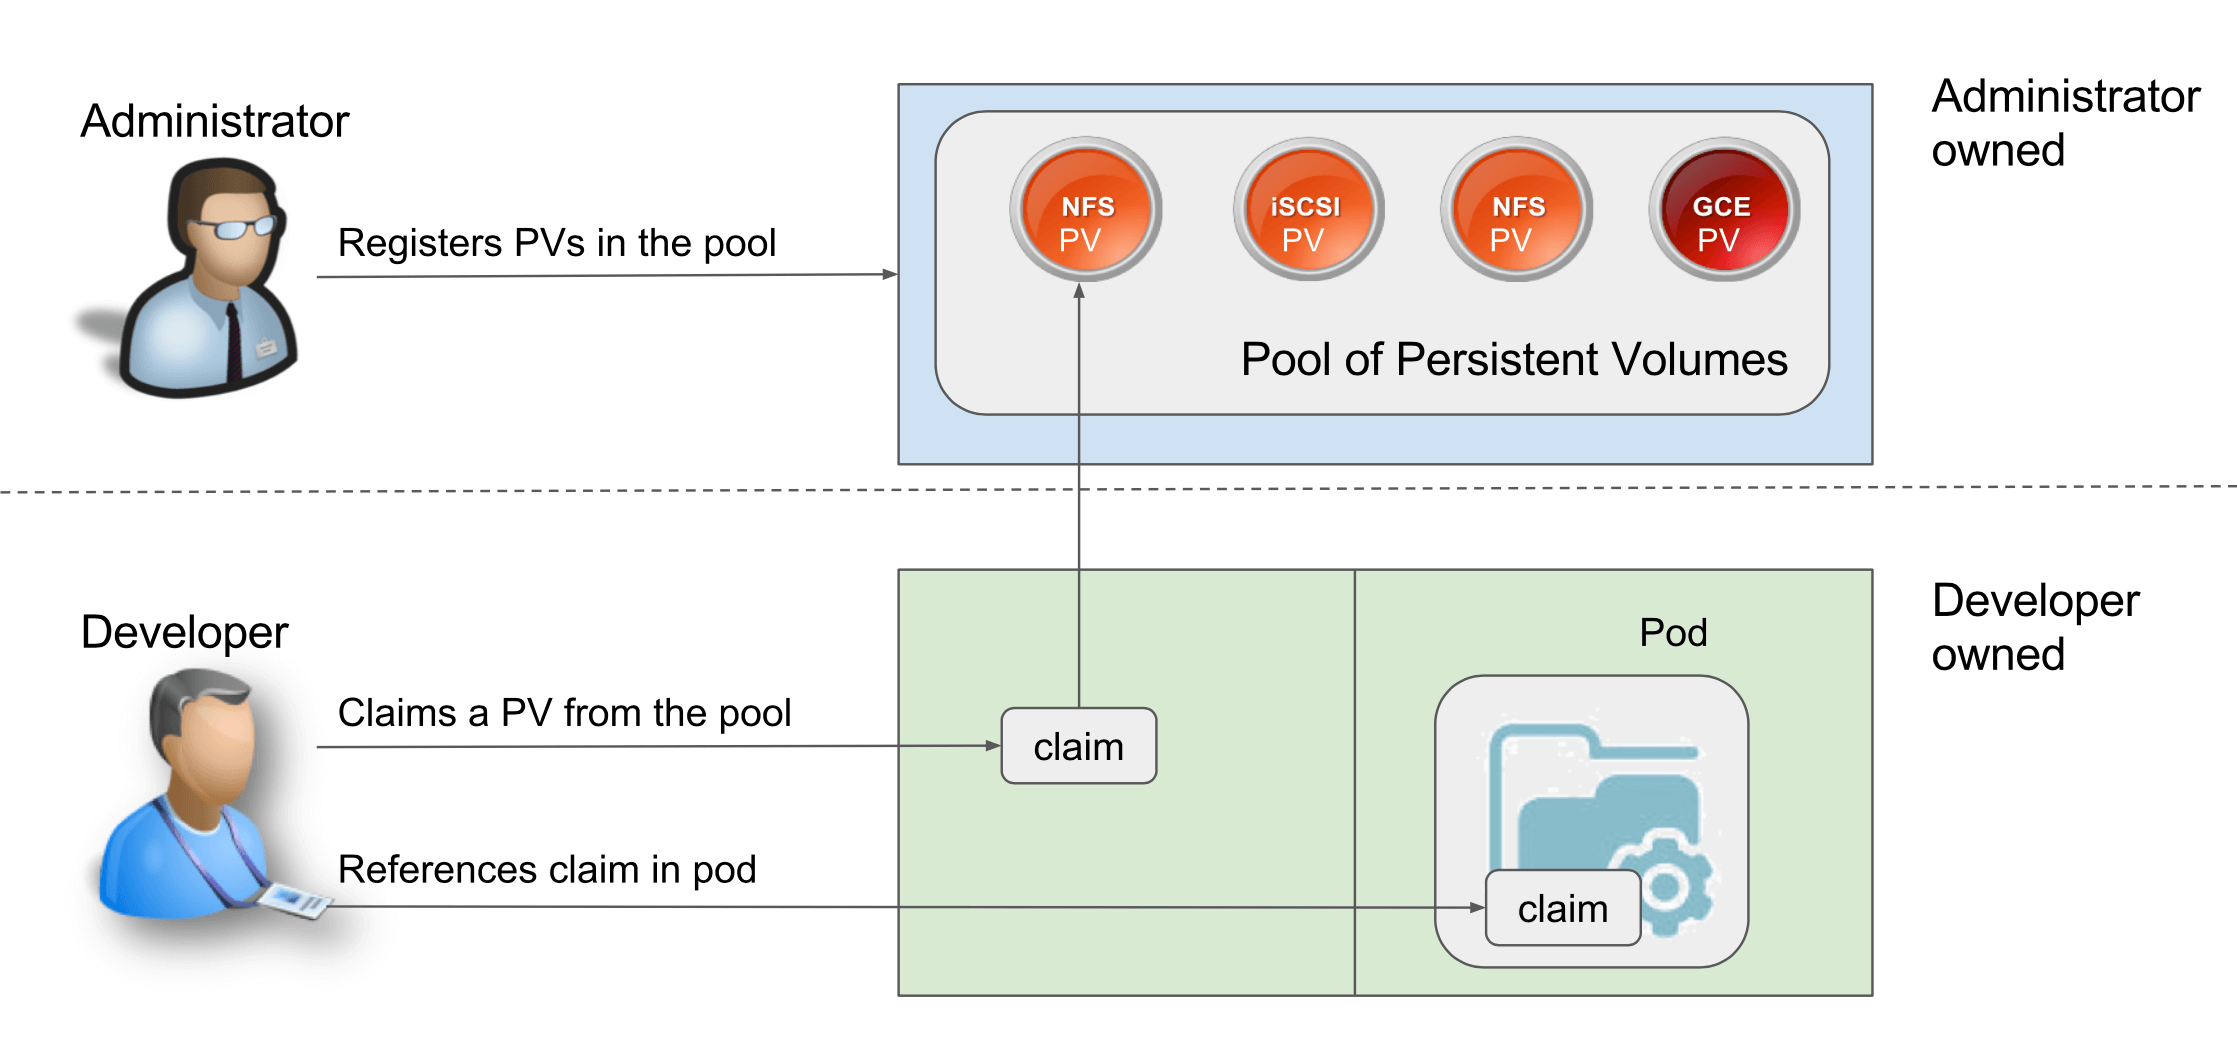
\includegraphics[scale=0.18]{kubernetes_pvc}
\caption{PersistantVolumeClaims management}
\end{figure}

It is important to understand the difference between \textbf{Volumes} and
\textbf{PersistantVolumes}/\textbf{PersistantVolumeClaims}. The former is
something like Docker volumes, used for persistence, host-based or on external
block storage devices but a user does not expect the resources to be reserved
before using it. In persistent volumes and claims, there is a strict enforcement
of resource utilization dictated by the policy defined during the creation of
resources. Kubernetes Pods can use claims as volumes.

\textbf{StorageClasses}\footnote{more information on different provisioners,
  policies and parameters can be found here: \\\url{
 https://kubernetes.io/docs/concepts/storage/storage-classes/ }} are a way to
describe different type of storage that can be used. Different classes can be
used to describe different levels of service or policies. PVCs that do not
specify a particular class can use the default one: to define it is possible to
use the annotation \verb!"storageclass.kubernetes.io/is-default-class":"true"!,
as for instance:

\begin{lstlisting}[language=bash]
kubectl patch storageclass glusterfs-storage -p '{"metadata": {"annotations":{"storageclass.kubernetes.io/is-default-class":"true"}}}'
\end{lstlisting}

\subsection{Volume and claim lifecycles}
\label{lifecycle}

We are going to briefly explain all the possible interactions between PVs and
PVCs.

\begin{enumerate}
\item \textbf{Provisioning}: there are 2 ways: statically or dynamically.
  \emph{Static} means that an administrator creates some PVs that are available
  for consumption. \emph{Dynamic} means that the cluster dynamically tries to
  provide a volume that matches a PVC. This is done with \emph{StorageClasses}:
  a claim requests storage for a certain storage class that can be provisioned.
  The class \texttt{""} disable dynamic provisioning;
\item \textbf{Binding}: a user requests a certain amount of storage with a claim
  and a control loop in the master looks for a PV that can bind the claim. In
  case of dynamic provisioning the loop always binds a PVC to a PV, otherwise
  the user will always get at least what they asked for, but the volume may be
  larger. Claims can remain unbound if a matching volume does not exists.
\item \textbf{Using}: after the binding phase the Pod starts using the volume
  (PVC is described in the Pod yaml
  \footnote{\url{https://kubernetes.io/docs/concepts/storage/persistent-volumes/\#claims-as-volumes}})
\item \textbf{Releasing}: when an application is done using the volume,
  developers can delete the PVC objects through the API, releasing the claim.
  This step will initiate the reclamation process.
\item \textbf{Reclaiming}: this phase is defined as a policy by the
  administrators. The reclaim policy for a PersistantVolume tells the cluster
  what to do with the volume after it has been released of its claim. Persistent
  volumes can either be \emph{retained}, \emph{recycled} or \emph{deleted}.
\end{enumerate}

\section{Installing Kubernetes}
\label{installing-kubernetes}

We performed our Kubernetes installation in a Openstack environment. Since we
used the Openstack of our school department, the administrators have given us a
virtual machine, \verb!Openstack-CLI!, to perform operations. From now, our
scripts assume to be in a machine with access to Openstack, and that the file
\verb!openrc.sh! has been sourced in the command line interface before
continuing. To install Kubernetes on CentOS 7 we develop a
script\footnote{available at
  \url{https://github.com/Augugrumi/init-script/tree/centos/kubernetes}}. With
CentOS is possible to have a complete installation with a
GlusterFS-PersistentStorage correctly set. After there is an explanation for the
most important part of the scripts. The script \verb!on_openstack_cli.sh!
\footnote{\url{https://github.com/Augugrumi/init-script/raw/centos/kubernetes/on_openstack_cli.sh}}
main aim is to run other files retrieving information even using \texttt{nova}
commands. First of all the software dependencies have to be installed and for
this purpose the script \verb!install_kubectl_repo.sh!
\footnote{\url{https://raw.githubusercontent.com/Augugrumi/init-script/centos/kubernetes/install_kubectl_repo.sh}}
was created. After the software installation it calls another script and waits
until all the machines are ready to proceed to the next step. The other script
is \verb!bootstrap.sh!
\footnote{\url{https://raw.githubusercontent.com/Augugrumi/vagrantfiles/oldversion/kubernetes/centos/bootstrap.sh}}
whose aim is to configure the machine and to install all the necessary
software. The bootstrap script first \textbf{disables SELinux} on all machines 
(needed for Kubernetes networking):
\begin{lstlisting}
sudo setenforce 0
sudo sed -i --follow-symlinks 's/SELINUX=enforcing/SELINUX=disabled/g' /etc/sysconfig/selinux
\end{lstlisting}
and then it enables the \verb!br_netfilter! module (needed for Kubernetes
networking):
\begin{lstlisting}
sudo modprobe br_netfilter
sudo sh -c 'echo "1" > /proc/sys/net/bridge/bridge-nf-call-iptables'
\end{lstlisting}
The swap is then switched off with the following commands:
\begin{lstlisting}
sudo swapoff -a
sudo sed -i '/swap/d' /etc/fstab
\end{lstlisting}
and it finally adds \texttt{rbd}, \texttt{ip\_vs}, \texttt{ip\_vs\_rr},
\texttt{ip\_vs\_wrr}, \texttt{ip\_vs\_sh}, \texttt{dm\_snapshot},
\texttt{dm\_mirror} and \texttt{dm\_thin\_pool} to the modules that will be
loaded at the machine startup.
\begin{lstlisting}
sudo sh -c 'echo -e "rbd ip_vs ip_vs_rr ip_vs_wrr ip_vs_sh" >  
/etc/modules-load.d/ip_vs.conf'
sudo sh -c 'echo -e "dm_snapshot dm_mirror dm_thin_pool" >  
/etc/modules-load.d/gluster.conf'
\end{lstlisting}
It is important to note that the last 3 modules will be useful in case
\gluster{} will be installed in the system. In the end the script installs
\texttt{docker}, \texttt{device-mapper-persistent-data}, \texttt{lvm2},
\texttt{kubelet}, \texttt{kubectl}, \texttt{kubeadm} and it starts (and enables)
\texttt{docker} and \texttt{kubelet} services. After this the machines are
rebooted. Considering $M$ to be the set of machines that are going to be added
to the Kubernetes cluster, for each host that is part of $M$ a set of entries
corresponding of the hostname and the IP address of every other node in $M$ will
be added in the \texttt{/etc/hosts} file. Then the installation continues in the
\textbf{master} node, with the script \verb!on_master.sh!
\footnote{\url{https://raw.githubusercontent.com/Augugrumi/init-script/centos/kubernetes/on_master.sh}}.
The following command initiates the Kubernetes cluster:
\begin{lstlisting}
sudo kubeadm init --apiserver-advertise-address=<ip-of-the-master> 
--Pod-network-cidr=10.244.0.0/16 --ignore-preflight-errors cri | grep "kubeadm 
join" > /home/centos/joincommand
\end{lstlisting}
Saving in the \texttt{joincommand} file the command that it will be run on the
slave node to join the cluster. There are some considerations to keep in mind
though:
\begin{enumerate}
  \item \verb!--pod-network-cidr! value depends on which agent you want to use
    to configure Kubernetes network. We choose Flannel so we put
    \texttt{10.244.0.0/16};
  \item at the moment we do not know why some preflight errors came out by
    running the aforementioned command and in order to ignore them we added the
    \verb!--ignore-preflight-errors cri! flag to in order to complete the
    set-up.
\end{enumerate}
Next it is necessary to run the following commands to create a folder
needed by Kubernetes to properly work:
\begin{lstlisting}
mkdir -p $HOME/.kube
sudo cp -i /etc/kubernetes/admin.conf $HOME/.kube/config
sudo chown $(id -u):$(id -g) $HOME/.kube/config
\end{lstlisting}
It is now necessary to wait until all the Pods get initialized, and this
operation is performed using the \verb!kubectl get pods --all-namespaces! in an
automated fashion. The next step is to install
Flannel\footnote{\url{https://github.com/coreos/flannel}} in order to make
networking between pods working:
\begin{lstlisting}
kubectl apply -f https://raw.githubusercontent.com/coreos/flannel/master/Documentation/kube-flannel.yml
kubectl apply -f https://raw.githubusercontent.com/coreos/flannel/master/Documentation/k8s-manifests/kube-flannel-rbac.yml
\end{lstlisting}
Later it is possible to setup the dashboard to access Kubernetes resources
running:
\begin{lstlisting}
kubectl create serviceaccount dashboard -n default
  kubectl create clusterrolebinding dashboard-admin -n default \
   --clusterrole=cluster-admin \
   --serviceaccount=default:dashboard
  kubectl get secret $(kubectl get serviceaccount dashboard -o jsonpath="{.secrets[0].name}") -o jsonpath="{.data.token}" | base64 --decode >  secret.txt
  screen -dmS kubectl_proxy_screen bash
  screen -S kubectl_proxy_screen -X stuff "kubectl proxy
  "
\end{lstlisting}
The dashboard will be accessible on the port 8001 only on the master node and it
will typically be reachable at this URL:
\url{https://<master-ip>:<apiserver-port>/api/v1/namespaces/kube-system/services/https:kubernetes-dashboard:/proxy/}
To access the information available on the dashboard the token stored into the
file \texttt{secret.txt} present on the home of the master node is needed.
Finally, in order to make a node join the cluster you have to run the command
saved into the \texttt{joincommand} file that we created before.

\section{Persistent Storage}
\label{persistent-storage}

\subsection{Prerequisites}
\label{prerequisites}

\begin{itemize}
\item A working installation of Kubernetes
\item Python (2.7) installed and available on all Kubernetes nodes
\end{itemize}

\subsection{\gluster{}}
\label{glusterfs}

\begin{figure}[htbp]
\centering
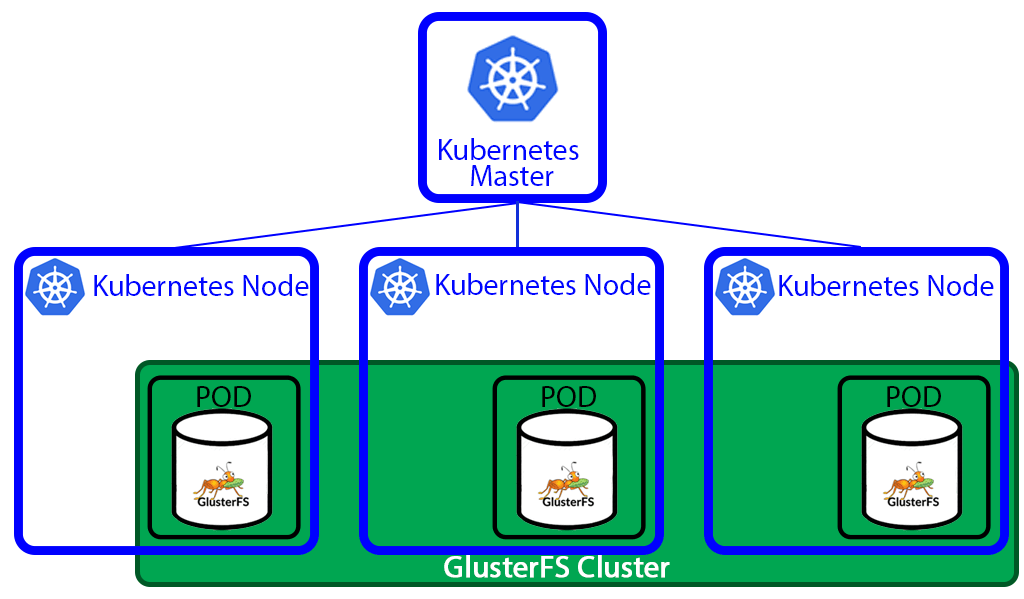
\includegraphics[scale=0.3]{glusterkube}
\caption{Installation of \gluster{} on Kubernetes cluster hosts}
\end{figure}

To enable persistent storage in Kubernetes with \gluster{} we need at least
three nodes. As described above, we deployed our Kubernetes cluster using CentOS
7\footnote{This procedure was tested on \texttt{Kubernetes\ v1.11.1.}}. Since we
are running our cluster on an Openstack environment, we attached a volume to
each VMs. First of all, you need to install \texttt{gluster-server} on all the
nodes that will join the storage and \texttt{gluster-fuse} to provide
\texttt{mount.glusterfs} as an option to mount \gluster{} file system. On a
command line interface we typed:
\begin{lstlisting}
sudo yum install -y centos-release-gluster && \
sudo yum install -y glusterfs-server glusterfs-fuse
\end{lstlisting}
The next step is to load different kernel modules, using \texttt{modprobe}:
\begin{lstlisting}
sudo sh -c 'modprobe dm_snapshot && modprobe dm_mirror && modprobe dm_thin_pool'
\end{lstlisting}
To make this change permanent, a new file
\texttt{/etc/modules-load.d/gluster.conf} needs to be created, with the
following content:
\begin{lstlisting}
dm_snapshot
dm_mirror
dm_thin_pool
\end{lstlisting}
At this point, you can make \texttt{glusterd} daemon run at system start up by
the command:
\begin{lstlisting}
sudo systemctl start glusterd && sudo systemctl enable glusterd
\end{lstlisting}
All the nodes on which you want to install \gluster{} must be labelled by
Kubernetes running the command:
\begin{lstlisting}
kubectl label node <node name> storagenode=glusterfs
\end{lstlisting}
According to the \emph{gluster-kubernetes setup guide}
\footnote{\url{https://github.com/gluster/gluster-kubernetes/blob/master/docs/setup-guide.md}},
the ports $2222$, $24007$, $24008$ and ports between $49152$ and $49251$ have to
be reachable. On top of that, you have to to grant access to your root account
during the installation of all the \gluster{} software. In CentOS you need to
access every machine and type:
\begin{lstlisting}
sudo su
cd /root/
nano .ssh/authorized_keys
# edit the first line in the follwing way: from the sub-string starting
# as "ssh-rsa" until the end put the content in a new line, while comment
# the whole line
nano /etc/ssh/sshd_config # un-comment "PermitRootLogin: yes"
systemctl restart sshd
\end{lstlisting}
Later you need to clone the \texttt{gluster-kubernetes} repository that contains
the script \texttt{gk-deploy}. It figures out all the necessary stuff (e.g.
heketi):
\begin{lstlisting}
git clone https://github.com/gluster/gluster-kubernetes.git
cd gluster-kubernetes/deploy
\end{lstlisting}
Then, we need to define the topology. To do so, a \texttt{topology.json}
file must be created. It can be done modifying the sample file
\texttt{topology.json.sample} with your topology, like in the following example:
\begin{lstlisting}
{
 "clusters": [
   {
     "nodes": [
       {
         "node": {
           "hostnames": {
             "manage": [
               "192.168.29.26"
             ],
             "storage": [
               "192.168.29.26"
             ]
           },
           "zone": 1
         },
         "devices": [
           "/dev/vdb"
         ]
       },
       {
         "node": {
           "hostnames": {
             "manage": [
               "192.168.29.19"
             ],
             "storage": [
               "192.168.29.19"
             ]
           },
           "zone": 1
         },
         "devices": [
           "/dev/vdb"
         ]
       },
       {
         "node": {
           "hostnames": {
             "manage": [
               "192.168.29.22"
             ],
             "storage": [
               "192.168.29.22"
             ]
           },
           "zone": 1
         },
         "devices": [
           "/dev/vdb"
         ]
       }
     ]
   }
 ]
}
\end{lstlisting}
After it is possible to deploy a \gluster{} cluster. On master the following
command must be run:
\begin{lstlisting}[language=bash]
# assuming you still are in ~/blabla/gluster-kubernetes/deploy/
./gk-deploy -s <path/to/your/private/key> --ssh-user root --ssh-port 22 topology.json -y
\end{lstlisting}
At the end of the script, if no error occurs, you can find a 
\texttt{StorageClass} definition file called \texttt{storageclass.yaml} and to
add the \texttt{StorageClass} to Kubernetes you have to type:
\begin{lstlisting}[language=bash]
kubectl create -f storageclass.yaml
\end{lstlisting}
Optionally, it can be set as default \texttt{StorageClass} with the following
command:
\begin{lstlisting}[language=bash]
kubectl patch -f storageclass.yaml \
-p'{"metadata": {"annotations":{"storageclass.kubernetes.io/is-default-class":"true"}}}'
\end{lstlisting}

\section{Ingress}
\label{ingress}

Ingresses allow services to be available from outside the cluster. There are 
different ways with which Kubernetes can handle service reachability, and these
are:
\begin{description}
  \item [ClusterIP:] Exposes the service on a cluster-internal IP. This value
    makes the service only reachable from within the cluster and is the default
    ServiceType value.
  \item [NodePort:]
  \footnote{\url{https://kubernetes.io/docs/concepts/services-networking/service/\#nodeport}}
  Exposes the service on each Node IP at a static port (the NodePort). A
  ClusterIP service, to which the NodePort service will route, is automatically
  created. It will be possible to contact the NodePort service, from outside the
  cluster, by requesting
  \texttt{\textless{}NodeIP\textgreater{}:\textless{}NodePort\textgreater{}}.
  \item [LoadBalancer:]
  \footnote{\url{https://kubernetes.io/docs/concepts/services-networking/service/\#loadbalancer}}
  Exposes the service externally using a load balancer of a cloud provider.
  NodePort and ClusterIP services, to which the external load balancer will
  route, are automatically created.
  \item [ExternalName:]
  \footnote{\url{https://kubernetes.io/docs/concepts/services-networking/service/\#externalname}}
  Maps the service to the contents of the ExternalName field
  (e.g.~foo.bar.example.com), by returning a CNAME record with its value. No
  proxying of any kind is set up. This requires version 1.7 or higher of
  \texttt{kube-dns}.
\end{description}
Since for the \texttt{LoadBalancer} typology we would need a Cloud service like 
AWS or GCE, we opted for the \texttt{NodePort} one. This is not a suitable
solution for production environments since it opens a couple of ports for every
Pods that runs in a node, but since we are building a test environment this
was considered to be fine.

Plenty of \texttt{ingresses-controllers} are available in the market and we
decided to analyze some of them.

\subsection{Nginx}
\label{nginx}
Kubernetes supports its own version of Nginx\footnote{
\url{https://github.com/kubernetes/ingress-nginx}}, but there is also an
ingress-controller supported by the official Nginx team\footnote{
\url{https://github.com/nginxinc/kubernetes-ingress}}.
We have chosen the second one, since it seems more stable.

\subsubsection{Installation}
\label{installation}

The installation is pretty simple, and it can be done with Helm:
\begin{lstlisting}[language=bash]
git clone https://github.com/nginxinc/kubernetes-ingress.git --depth 1 # Clone the project repository
kubernetes-ingress/helm-chart
helm install --name nginxcontroller . --set controller.replicaCount=2,controller.service.type=NodePort,controller.service.externalTrafficPolicy=Cluster # Install the helm package
\end{lstlisting}
At this point, if you want to expose a service you need to create a file
similar to this one:
\begin{lstlisting}[language=yaml]
apiVersion: extensions/v1beta1
kind: Ingress
metadata:
 name: wordpress-ingress
spec:
 rules:
 - host: wordpress.example.com
   http:
     paths:
     - path: /<your-url-path>
       backend:
         serviceName: <your-service-name>
         servicePort: 80
\end{lstlisting}
And apply your forwarding to Kubernetes running the command:
\begin{lstlisting}[language=bash]
kubectl create -f ingress-forwarding.yaml
\end{lstlisting}
In the dashboard, you should see now something similar to this:
\begin{figure}[htbp]
\centering
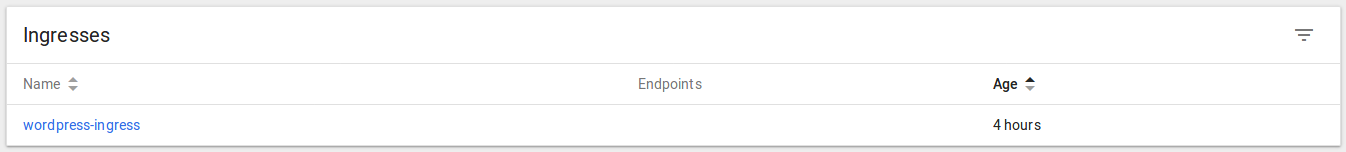
\includegraphics[scale=0.3]{ingress}
\caption{Example of ingress in Kubernetes dashboard}
\end{figure}

\subsection{Træfik}
\label{truxe6fik}

\subsubsection{Installation}
\label{installation-1}
Role based access control was introduced in Kubernetes 1.6 and to make Træfik
working properly it must be configured. For simplicity, ClusterRoleBinding can
be used as in the Træfik installation guide\footnote{
\url{https://docs.traefik.io/user-guide/kubernetes/}}:
\begin{lstlisting}[language=yaml]
---
kind: ClusterRole
apiVersion: rbac.authorization.k8s.io/v1beta1
metadata:
  name: traefik-ingress-controller
rules:
  - apiGroups:
      - ""
    resources:
      - services
      - endpoints
      - secrets
    verbs:
      - get
      - list
      - watch
  - apiGroups:
      - extensions
    resources:
      - ingresses
    verbs:
      - get
      - list
      - watch
---
kind: ClusterRoleBinding
apiVersion: rbac.authorization.k8s.io/v1beta1
metadata:
  name: traefik-ingress-controller
roleRef:
  apiGroup: rbac.authorization.k8s.io
  kind: ClusterRole
  name: traefik-ingress-controller
subjects:
- kind: ServiceAccount
  name: traefik-ingress-controller
  namespace: kube-system
\end{lstlisting}
Save that in a file \texttt{traefik-rbac.yaml} and run:
\begin{lstlisting}[language=bash]
kubectl apply -f traefik-rbac.yaml
\end{lstlisting}
After the ingress controller can be set up in to two different way: using a
Deployment or a DaemonSet. We chose the first option for easier management. We
deployed it with this YAML:
\begin{lstlisting}[language=yaml]
---
apiVersion: v1
kind: ServiceAccount
metadata:
  name: traefik-ingress-controller
  namespace: kube-system
---
kind: Deployment
apiVersion: extensions/v1beta1
metadata:
  name: traefik-ingress-controller
  namespace: kube-system
  labels:
    k8s-app: traefik-ingress-lb
spec:
  replicas: 1
  selector:
    matchLabels:
      k8s-app: traefik-ingress-lb
  template:
    metadata:
      labels:
        k8s-app: traefik-ingress-lb
        name: traefik-ingress-lb
    spec:
      serviceAccountName: traefik-ingress-controller
      terminationGracePeriodSeconds: 60
      containers:
      - image: traefik
        name: traefik-ingress-lb
        ports:
        - name: http
          containerPort: 80
        - name: admin
          containerPort: 8080
        args:
        - --api
        - --kubernetes
        - --logLevel=INFO
---
kind: Service
apiVersion: v1
metadata:
  name: traefik-ingress-service
  namespace: kube-system
spec:
  selector:
    k8s-app: traefik-ingress-lb
  ports:
    - protocol: TCP
      port: 80
      name: web
    - protocol: TCP
      port: 8080
      name: admin
  type: NodePort
\end{lstlisting}
As before, save it in a file, say \texttt{traefik-deployment.yaml} and run:
\begin{lstlisting}[language=bash]
kubectl apply -f traefik-deployment.yaml
\end{lstlisting}
This deployment will expose two \texttt{NodePorts} services that allow to access
to the ingress and to the web management interface.

\section{Additional Tools}
\label{additional-tools}

\subsection{Helm}
\label{helm}

To install Helm you need to be in the master node\footnote{
\url{https://docs.helm.sh/using_helm/\#installing-helm}} and run the
command:
\begin{lstlisting}[language=bash]
curl https://raw.githubusercontent.com/kubernetes/helm/master/scripts/get | bash
\end{lstlisting}
To make it working correctly you should give it some additional permission
creating a file like this:
\begin{lstlisting}[language=yaml]
apiVersion: v1
kind: ServiceAccount
metadata:
  name: helm
  namespace: kube-system
---
apiVersion: rbac.authorization.k8s.io/v1beta1
kind: ClusterRoleBinding
metadata:
  name: helm
roleRef:
  apiGroup: rbac.authorization.k8s.io
  kind: ClusterRole
  name: cluster-admin
subjects:
  - kind: ServiceAccount
    name: helm
    namespace: kube-system
\end{lstlisting}
And after deploying the service running:
\begin{lstlisting}[language=bash]
kubectl create -f helm.yaml
\end{lstlisting}
At this point, we have defined a new ClusterRole, \emph{helm}, that has the
possibility to interact with \texttt{kube-system} namespace. Now we were able to
deploy Tiller in our cluster (Helm backend), by running:
\begin{lstlisting}[language=bash]
 helm init --service-account helm --wait
 \end{lstlisting}
